\section{Light Calibration During Detector Operation}
\label{secGainCalibration}


The analysis of the experimental data of XENON100 requires the detailed characterization of 242 individual channels. PMT calibration is performed regularly for this purpose, by stimulating single  photoelectron emission from the photocathode with a light-emitting diode (LED) light. The main goal of the light calibration is to measure the absolute gain of every channel, and monitor the response over time. Several additional parameters are also determined, such as the single photoelectron resolution, peak-to-valley, and signal-to-noise ratios.

A dedicated system has been developed for the light calibration of the PMTs in the XENON100 detector, including the hardware setup with an external LED source, and the analysis and monitoring software: ROOT-based C++ programs for the data processing and analysis of the single photoelectron response, a dynamic database, and a web-based visualization tool. 

%\subsection{Hardware Setup}
%\label{secGainCalibrationHardware}

%\begin{floatingfigure}[r]{0.6\textwidth}
\begin{figure}[!t]
\centering
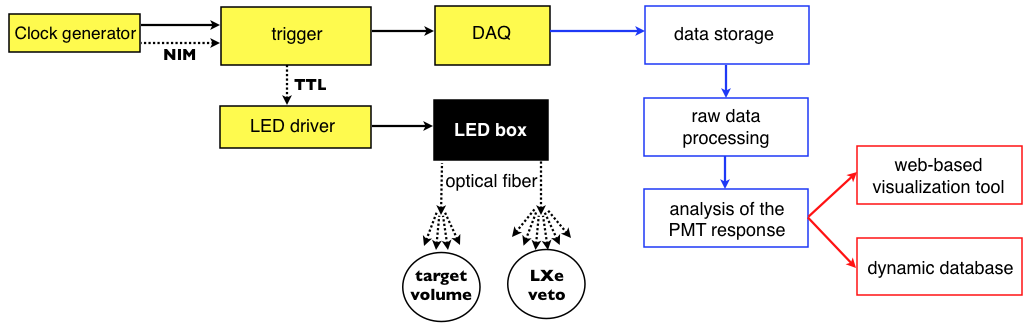
\includegraphics[width=1.0\linewidth]{plots/PMTcalibration/CalibrationSchemeFull.png}
\caption[Schematic of the setup for PMT calibration]{Schematic of the setup for PMT calibration, which consists of hardware setup with an external LED with the optical fiber light guides, and the analysis and monitoring software.}
\label{figCalibrationSetup}
\end{figure}
%\end{floatingfigure}

The hardware system for the PMT calibration with LEDs has been set up as shown in Fig.~\ref{figCalibrationSetup}. An external clock is connected to the DAQ trigger input with a NIM signal, and the TTL output is sent to the pulse generator (LED driver). The LED driver provides two output channels connected to a light-tight box with two InGaN LEDs, which emit blue light  with an average wavelength of 470~nm. The light from the LEDs is transferred by two standard coated optical fibers (1~mm core) to optical feedthroughs on the detector flange. At the vacuum side of the feedthroughs, two uncoated quartz fibers are connected (800~$\mu$m core), which direct the light into the detector volume. Quartz is chosen for its high melting point, which allows  the pipes to be baked at higher temperatures (up to 200$^{\circ}$C). In order to diffuse the light and to achieve a uniform illumination of all PMTs, the quartz fibers are connected inside the cryostat to two bundles of polymethylmethacrylate (PMMA-PFA) fibers with 180~$\mu$m core. PMMA-PFA optical fiber is more flexible than quartz, thus well suited for small bending radii inside the cryostat. The coating has been removed from the fibers, in order to minimize the amount of materials placed in liquid xenon. Temperature resistance is not crucial for these inner fibers, because the baking temperature is limited by the allowed range for the PMTs (50$^{\circ}$C). A `1-to-4' optical fiber bundle is used to illuminate top and bottom PMT arrays in the target volume, and a `1-to-6' bundle guides the light into the veto volume. Two branches of the veto bundle are used for PMTs on the top and bottom of the veto volume, and four remaining ones are used to illuminate the side veto PMTs.

%\begin{figure}[!h]
%\centering
%\subfigure[]{
%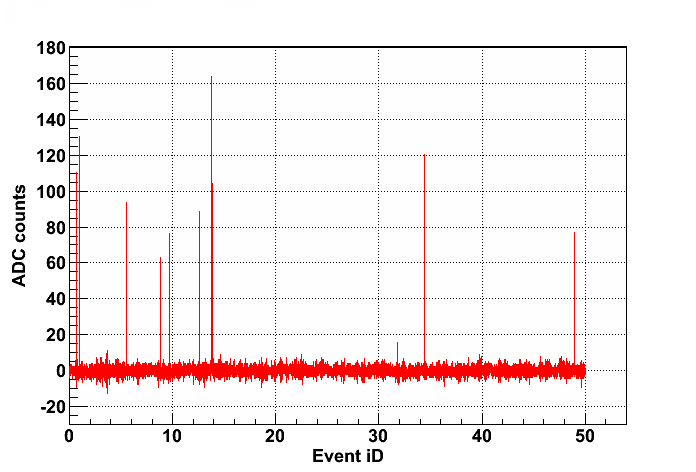
\includegraphics[width=0.475\linewidth]{plots/PMTcalibration/PMT131_wf.png}
%\label{figPMTwf_1}}
%\subfigure[]{
%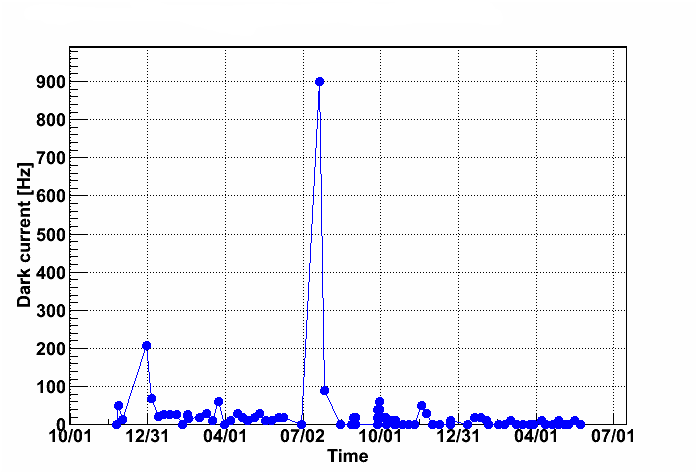
\includegraphics[width=0.475\linewidth]{plots/PMTcalibration/dc1_vs_time_PMT146.png}
%\label{figPMTwf_2}}
%\caption{(a) - a waveform of the PMT signal recorded during the calibration run, after baseline subtraction. (b) - a long-term dark current rate evolution for one of the XENON100 PMTs. }
%\label{figPMTwf}
%\end{figure}

The total amount of light produced by an LED depends on the amplitude of the voltage pulse and on its time width. In order to achieve single PE level for PMT illumination, the amplitude of the pulse has been set to the minimum required to turn on the LED. If the time delay between the light signals is shorter than the time necessary to restore the initial condition on each dynode, this might produce drift effects on the PMT gain. Thus, a relatively low pulse rate of 100~Hz is used, which still allows the acquisition of reasonable statistics in a short time: 100'000 events take about 20~min, with an average of $\sim$1'000 signal pulses per PMT. 

The width of the pulse is 4~$\mu$s, and the total digitization window is 5~$\mu$s. The data is acquired without zero length encoding. The DAQ has been set such that 1~$\mu$s (100 samples) is acquired before the trigger, in order to compute the baseline for each event by averaging the ADC counts. 
The signal rate in the pre-trigger part of the digitized waveform is additionally used to monitor `dark count' rate of the PMTs. Even though some signals are always present when the scintillator medium is present in the detector, this provides a possibility to monitor the PMT functionality. 
%The typical waveform of the PMT signal after baseline subtraction is shown in Fig.~\ref{figPMTwf_1}. 
% An example of the long-term dark current rate evolution for one of the XENON100 PMTs is shown in Fig.~\ref{figPMTwf_2}. 

Ideally, all PMTs should be uniformly illuminated, so that each phototube detects light on the level of single PE. Since the optical fibers for illumination of the inner PMTs are installed in the liquid phase, the light from an LED is reflected on the liquid surface, and the amount of light on the top array is significantly lower than on the bottom PMT array (Fig.~\ref{figLightLevel_1}). In addition, its maximum is not synchronized in time for both PMT arrays. The difference in light level is also present for the PMTs within the same array, due to geometrical effects and differences in the QE of the phototubes.
%The typical waveform of the PMT signal after baseline subtraction is shown in Fig.~\ref{figLightLevel_2}. 

%\begin{floatingfigure}[r]{0.6\textwidth}
\begin{figure}[!h]
\centering
\subfigure[]{
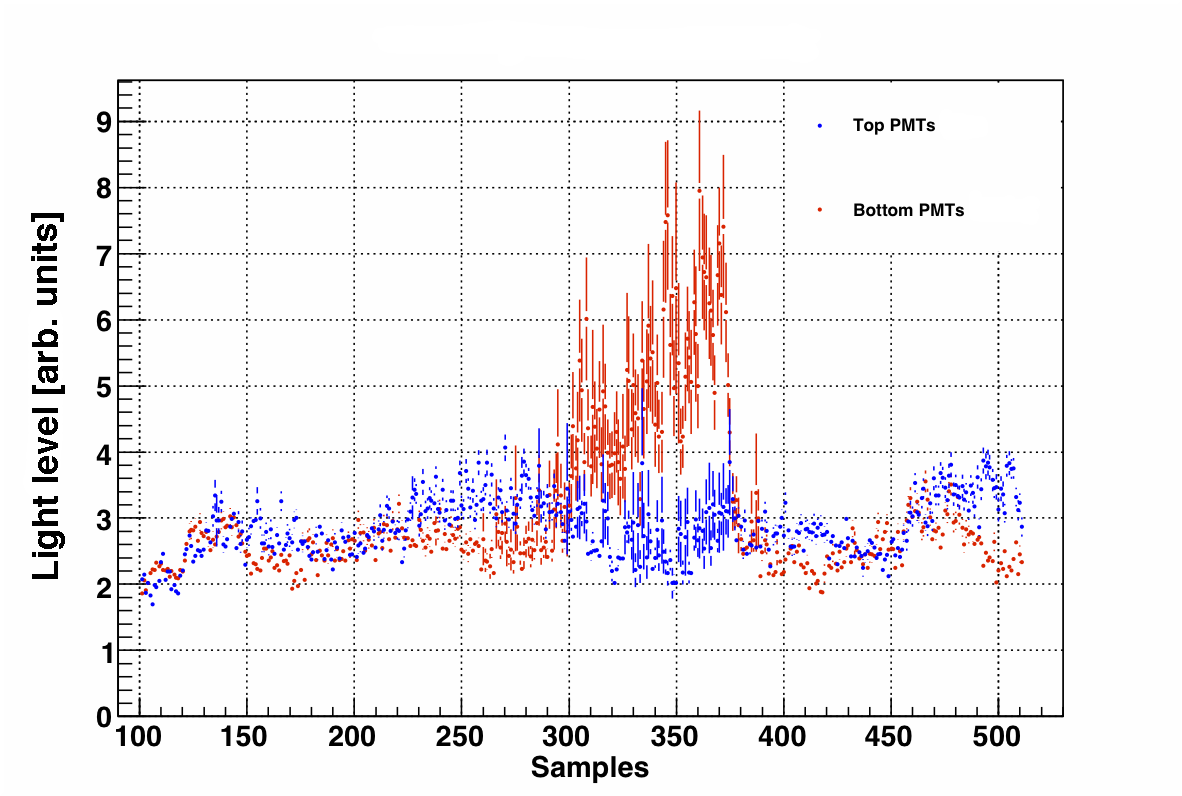
\includegraphics[width=0.475\linewidth]{plots/PMTcalibration/ADCvsSMPmod.png}
\label{figLightLevel_1}}
\subfigure[]{
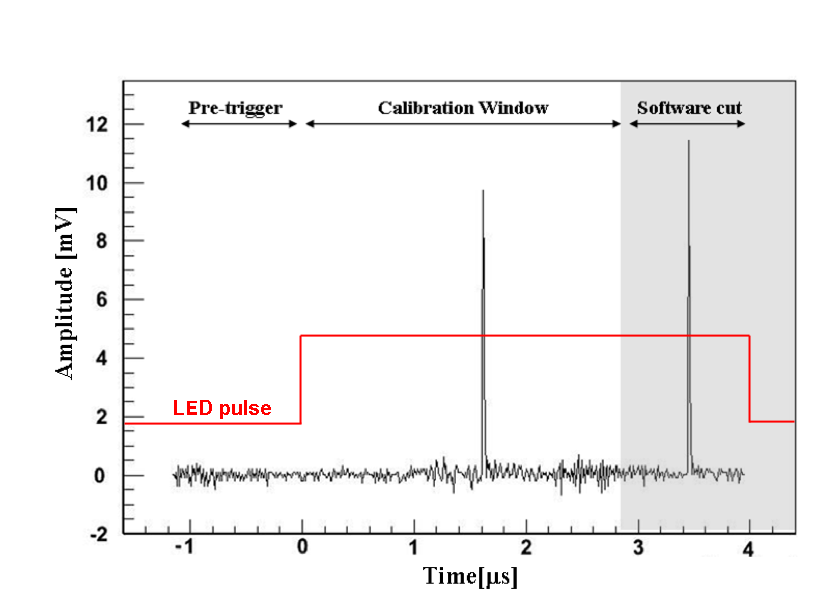
\includegraphics[width=0.47\linewidth]{plots/PMTcalibration/PMTcalibrationWindow_withLEDpulse.png}
\label{figLightLevel_2}}
\caption[Light level on the top and bottom PMT arrays in the target volume, and a typical waveform of the PMT signal]{(a) - Light level on the top and bottom PMT arrays in the target volume as a function of the data acquisition time within one event; 1~sample~=~10~ns. (b) - a typical waveform of the PMT signal, with an indicated software cut for the pulse search window.}
\label{figLightLevel}
\end{figure}
%\end{floatingfigure}

In order to equalize the amount of light detected by each phototube, a software cut on the calibration window size has been developed, which allows reduction of multiple PE emission within one event (Fig.~\ref{figLightLevel_2}). The number of samples in the calibration window shown in Fig.~\ref{figLightLevel_2} is adjusted for each PMT in such a way that the ratio of the number of triggers with no detected signal and the total number of triggers does not exceed 95\%. Brightly illuminated PMTs have a short search window, and dimly illuminated a longer one, up to full length of the LED pulse (4~$\mu$s).

%\begin{figure}[!h]
%\centering
%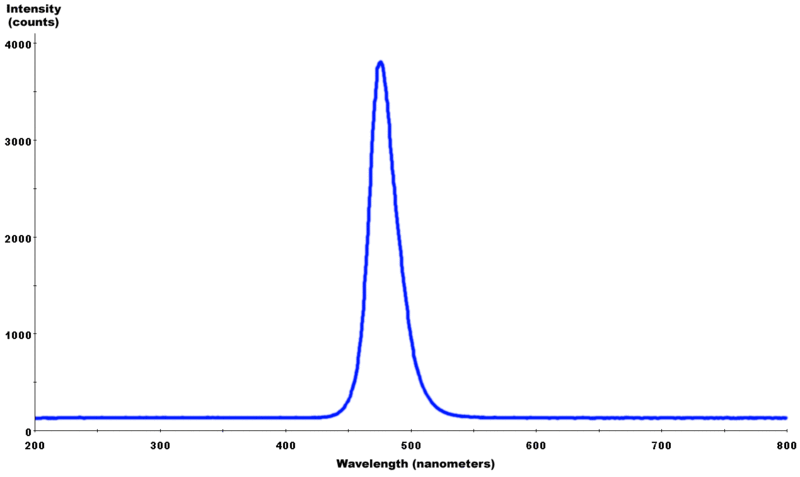
\includegraphics[width=0.5\linewidth]{plots/PMTcalibration/BlueLEDSpectrum.png}
%\caption{Spectral response of InGaN ('blue') LED.}
%\label{figLEDspectrum}
%\end{figure}

%\subsection{Analysis and Monitoring Software}
%\label{secGainCalibrationSoftware}

The first stage of the data analysis includes processing of the raw data, which produces a ROOT file storing the content in ADC counts of 10 bins across the maximum with subtracted baseline.

At the second stage, the pulse area is calculated from the integrated pulse height, and the PMT response is analyzed. An example of the spectrum induced by the LED light is shown as integrated ADC counts in Fig.~\ref{figPMTresponse_1}. The response of the PMT is described by a sum of two functions, describing the noise peak (pedestal), and single PE peak. The noise peak is usually fitted by a Gaussian function, and the single PE peak is described by a continuous distribution in the form~\cite{SPEfit1, SPEfit2}:
\begin{equation}
\label{ContinuousDistribution}
y = \frac{\mu^x \cdot e^{-\mu}}{\Gamma[x+1]},
\end{equation}
where $y$ is the number of counts/channels in the spectrum, $x$ is the ADC value, $\mu$ is the mean of the Poisson distribution, and $\Gamma$ is the gamma function, given by:
\begin{equation}
\label{GammaFunction}
\Gamma[x] = \int t^{x-1}\ e^{-t}\ dt.
\end{equation}

The integrated ADC counts are converted to PMT gain as following:

\begin{equation}
\mathrm{gain} = \frac{\mu \cdot r}{Z \cdot A \cdot f \cdot e},
\end{equation}
where $\mu$ - mean of the single PE peak in ADC counts;
$r$~=~2.25/2$^{14}$~[V/bit] - ADC resolution;
$Z$~=~50~[Ohm] - input impedance; 
$A$~=~10 - amplification factor for PMT signal; 
$f$~=~10$^{8}$~[s$^{-1}$] - sampling frequency; 
$e$~=~1.60218$\cdot$10$^{-19}$~C - electron charge.

The typical dark current spectrum of a XENON100 PMT during detector operation is shown in Fig.~\ref{figPMTresponse_2}. The dark current is calculated in different ranges: for the pulses more than 6$\sigma$ away from noise peak, based on a Gaussian fit of the latter, for the pulses with an amplitude 200-700 ADC counts, 300-700 ADC counts, and $>$700 ADC counts.

\begin{figure}[!h]
\centering
\subfigure[]{
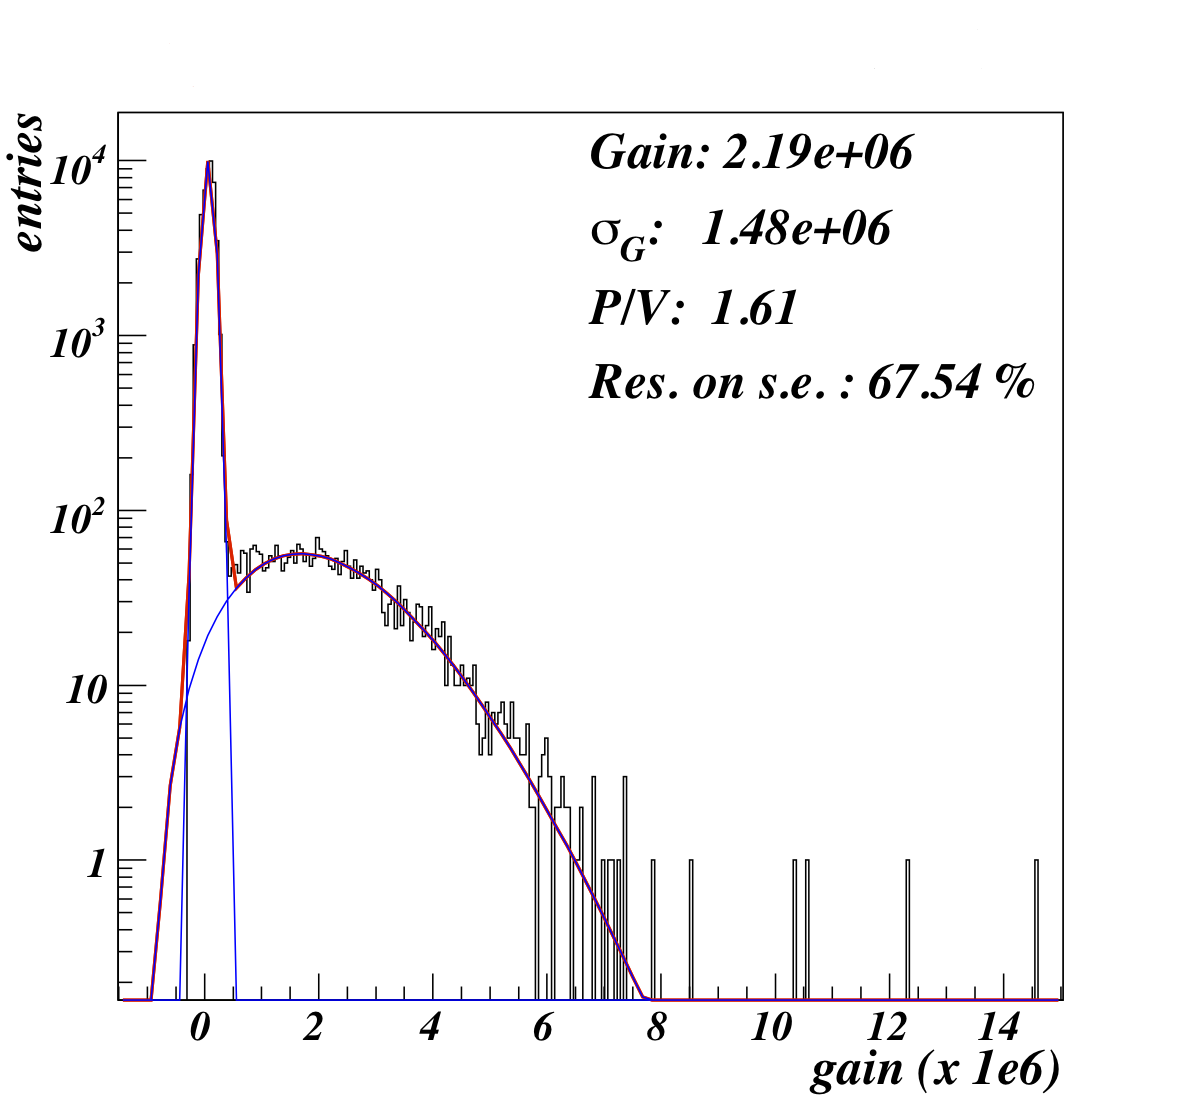
\includegraphics[height=0.4\linewidth]{plots/PMTcalibration/PMTsinglePE.png}
\label{figPMTresponse_1}}
\subfigure[]{
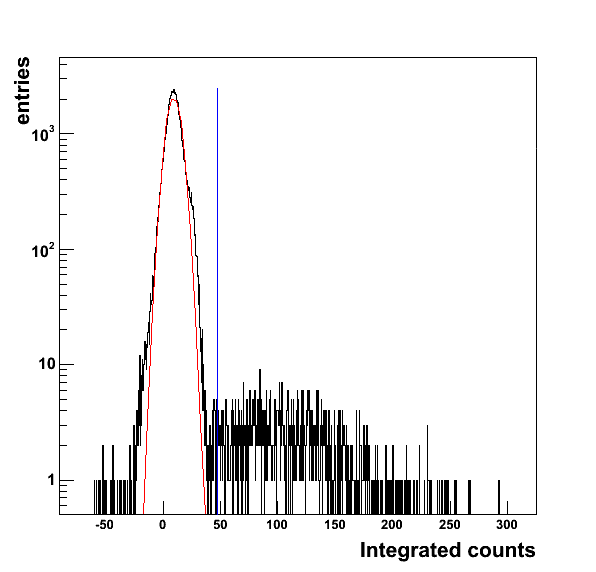
\includegraphics[height=0.4\linewidth]{plots/PMTcalibration/PMTdc_clean.png}
\label{figPMTresponse_2}}
\caption[Response of a XENON100 PMT to an LED light and a typical dark current spectrum]{Response of a XENON100 PMT to an LED light (a) and a typical dark current spectrum (b).}
\label{figPMTresponse}
\end{figure}

For most of the PMTs, a Gaussian function is a good approximation of the noise distribution. However, on some of the channels electronic noise with different amplitudes and frequencies has been observed. In this case, the random position and width of the PMT pulses at the pedestal peak does not allow use of a general function to fit the noise part of the spectrum. The origin of the electronic noise is a pick-up on high voltage line, thus the noise is correlated on the channels which are connected through to the same HV board or filter box. The light signal on all channels is on the contrary not correlated, which provides a method to discriminate electronic noise. Such noise removal technique is used for the PMTs 1 and 2, installed in the top PMT array (see Fig.~\ref{figNoiseDiscrimination_1}). The spectrum of the PMT1 is shown with a blue histogram in Fig.~\ref{figNoiseDiscrimination_2}. The amplitude and frequency of the electronic noise on this channel are so high that it significantly overlaps with the signal distribution, and the PMT gain cannot be determined. Using the cut on the correlation of the pulse height between channels 1 and 2, it is possible to completely remove the noise population and get the clean single PE distribution. However, some part of low amplitude signal pulses are removed, and the measured gain is biased to slightly higher values.

\begin{figure}[!h]
\centering
\subfigure[]{
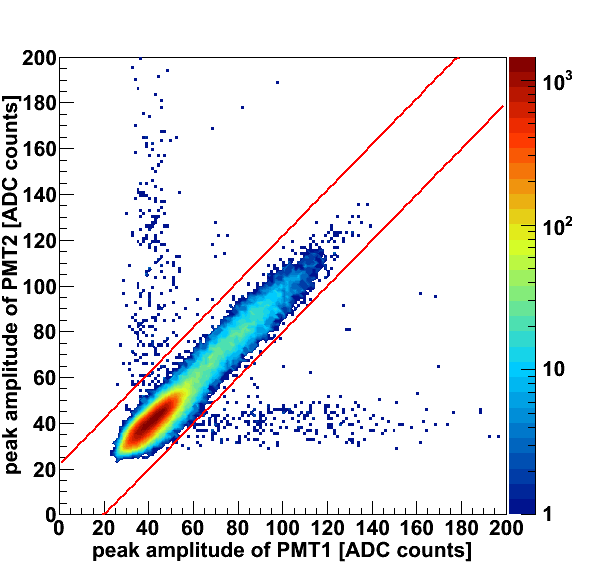
\includegraphics[height=0.4\linewidth]{plots/PMTcalibration/CorrelatedNoise_PMT1-2.png}
\label{figNoiseDiscrimination_1}}
\subfigure[]{
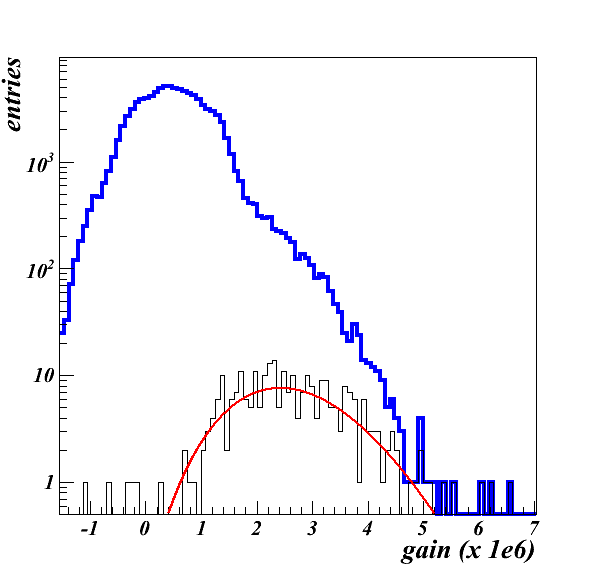
\includegraphics[height=0.4\linewidth]{plots/PMTcalibration/PMT1_withNoiseCut.png}
\label{figNoiseDiscrimination_2}}
\caption[Discrimination of the correlated electronic noise]{Discrimination of the correlated electronic noise: (a) - discrimination parameter; (b) - spectrum of PMT1 without (blue) and with (black) noise cut, together with the single PE fit (red).}
\label{figNoiseDiscrimination}
\end{figure}

The gain calibration is performed weekly, and fits of all the 242 PMTs are visually inspected to ensure the fit quality. For this purpose, a web-based tool with an interactive PMT map has been developed. The output of the analysis is written into a dynamic MySQL database, which allows the data processing software to automatically take into account changes in the PMT characteristics. 

The gains of all PMTs in the XENON100 detector have been equalized to approximately 2$\times$10$^{6}$ (Fig.~\ref{figGainDistribution_1}), which corresponds to an average area of a single PE peak of $\sim$120 ADC counts. An example of the long-term stability of the PMT gain is shown in Fig.~\ref{figGainDistribution_2}. The average gain of the XENON100 PMTs is 1.96$\times$10$^{6}$ with the differences between the channels on the order of 10\%, and is stable over time within $\pm$2\% ($\sigma/\mu$), which is comparable with the statistical error of the gain determination (1.6\%). The distribution of the peak-to-valley ratio is centered at 52\%, and the resolution on the single PE is on average 52\%.

\begin{figure}[!h]
\centering
\subfigure[]{
%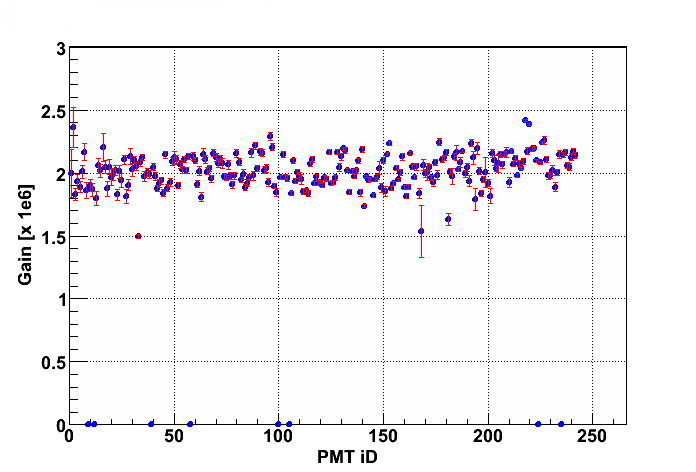
\includegraphics[width=0.475\linewidth]{plots/PMTcalibration/gr_gain.png}
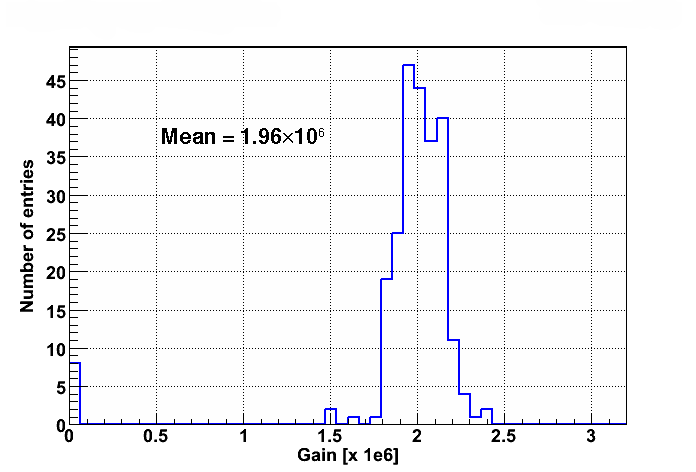
\includegraphics[width=0.475\linewidth]{plots/PMTcalibration/h_gain1.png}
\label{figGainDistribution_1}}
\subfigure[]{
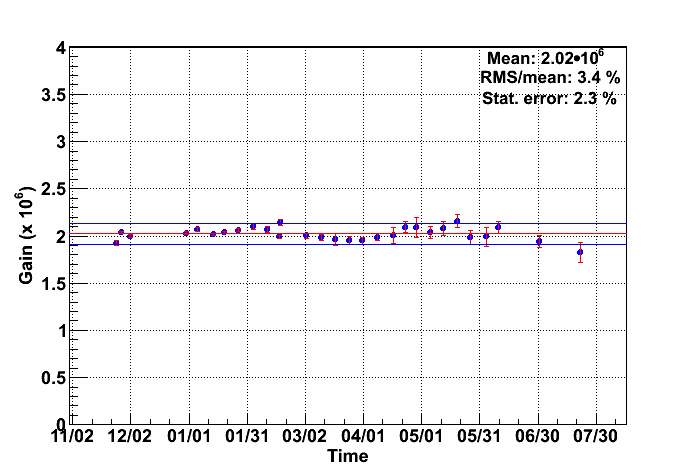
\includegraphics[width=0.475\linewidth]{plots/PMTcalibration/gain_vs_time.png}
\label{figGainDistribution_2}}
\caption[The equalized gains of the XENON100 PMTs and an example of the long-term stability]{The equalized gains of the XENON100 PMTs (a) and an example of the long-term stability for one of them (b). The horizontal blue lines indicate the RMS  spread over an 8 month period. It is comparable with the statistical errors of the measurements.}
\label{figGainDistribution}
\end{figure}


% , because it is  A methods have been developed in order to discriminate the electronic noise on such PMTs.

% One of them is based on pulse shape analysis of the digitized waveform, using as a discrimination parameter the ratio between the height of the peak and the summed counts in the integration window (Fig.~\ref{figNoiseDiscrimination}). However, such a cut removes together with noise the signal pulses with lower amplitude, and the gain calculated with this method is biased towards higher values. The second method is used for the channels on which the noise is 




%`

